\chapter{Implementierung der Kernfunktionen}
\label{ch:implementierung_kernfunktionen}
Aufbauend auf den technologischen Entscheidungen und der Systemarchitektur, die im vorherigen Kapitel~\ref{ch:systemarchitektur} definiert wurden, widmet sich dieses Kapitel der praktischen Umsetzung von \textit{EffSync}. Der Fokus liegt dabei auf der Implementierung der wesentlichen Kernfunktionen.

Im Folgenden wird detailliert erläutert, wie zentrale Features, wie beispielsweise das Task-Management, die Echtzeitkommunikation und die rollenbasierte Zugriffssteuerung, technisch realisiert wurden. Anhand ausgewählter Abläufe wird demonstriert, wie das Vue.js-Frontend und das NestJS-Backend in der Praxis zusammenarbeiten.

\authorsection{Authentifizierung}{Ereny Micail}
\label{sec:authentifizierung}
Die Authentifizierung in \textit{EffSync} stellt sicher, dass ausschließlich registrierte Benutzer auf geschützte Ressourcen zugreifen können. Nach erfolgreichem Login wird ein Zugriffstoken ausgestellt, das bei nachfolgenden API-Aufrufen im \texttt{Authorization}-Header übertragen wird. Das Backend validiert dieses Token serverseitig, bevor Controller-Methoden für geschützte Endpunkte ausgeführt werden.


Zur Absicherung gegen Missbrauch wird zusätzlich ein Request-Throttling eingesetzt. Sicherheitsrelevante Endpunkte wie die Registrierung werden limitiert, sodass wiederholte Anfragen in kurzer Zeit automatisch mit HTTP \texttt{429 Too Many Requests} blockiert werden. Die Wirksamkeit dieses Mechanismus wird durch E2E-Tests verifiziert.

Neben der klassischen Anmeldung mit Benutzername/E-Mail und Passwort unterstützt \textit{EffSync} auch einen OAuth-2.0-basierten Login über Google. Ziel dieser Erweiterung ist es, den Zugang zur Plattform für Benutzer zu vereinfachen und gleichzeitig die Sicherheit der Anmeldung durch einen etablierten externen Identity-Provider zu erhöhen.

Technisch wird der OAuth-Flow über \texttt{Passport} und die Strategie \texttt{passport-google-oauth20} in das NestJS-Backend integriert. Der Ablauf folgt dem üblichen Prinzip:
\begin{enumerate}
    \item Der Benutzer startet den Login über den Google-Provider.
    \item Nach erfolgreicher Authentifizierung bei Google wird der Benutzer zum Backend zurückgeleitet.
    \item Das Backend validiert die Provider-Daten, ordnet den Account einem bestehenden Benutzer zu bzw. legt einen neuen an.
    \item Anschließend wird für die weitere API-Nutzung ein eigener Anwendungstoken ausgestellt.
\end{enumerate}

Damit bleibt die interne Autorisierungslogik von \textit{EffSync} konsistent: Unabhängig davon, ob der Benutzer über Passwort-Login oder OAuth einsteigt, erfolgen Rollen- und Berechtigungsprüfungen weiterhin ausschließlich innerhalb der Plattformlogik. OAuth erweitert somit den Authentifizierungsweg, ersetzt jedoch nicht das interne Berechtigungsmodell.


\authorsection{Rollen und Berechtigungen}{Ereny Micail}
\label{sec:rollen_berechtigungen}
Neben der reinen Authentifizierung implementiert \textit{EffSync} ein differenziertes Autorisierungskonzept. Berechtigungen werden nicht ausschließlich global über Rollen vergeben, sondern kontextabhängig auf Aufgabenebene ausgewertet. Dadurch kann das System präzise unterscheiden, ob ein Benutzer eine Aktion nur lesen, schreiben oder administrativ ausführen darf.

Technisch werden Berechtigungen in Form von Flags verarbeitet (z.\,B. \texttt{READ}, \texttt{WRITE}, \texttt{EXECUTE}). Diese lassen sich effizient kombinieren und prüfen, wodurch eine performante Rechteauswertung für API-Anfragen möglich ist. Zusätzlich können zeitliche Gültigkeitsgrenzen (\texttt{valid\_from}, \texttt{valid\_to}) berücksichtigt werden, um befristete Rechte kontrolliert abzubilden.

Besonders kritische Aktionen – wie das Hinzufügen oder Entfernen von Mitgliedern – werden serverseitig strikt validiert. Unzulässige Zugriffe werden konsistent mit HTTP \texttt{403 Forbidden} abgelehnt. Damit wird verhindert, dass Benutzer außerhalb ihres Verantwortungsbereiches Veränderungen an Aufgaben- oder Raumstrukturen vornehmen.

Zur administrativen Pflege dieses Rechtemodells steht Benutzern mit entsprechender Berechtigung ein eigenes Admin-Panel zur Verwaltung von Rollen und Berechtigungen zur Verfügung (siehe Abbildung~\ref{fig:admin_rollen_permissions}). Über die in der linken Seitenleiste hervorgehobene Zahnrad-Schaltfläche gelangt man in diesen Bereich. Dort lässt sich pro Benutzer einsehen und bearbeiten, welche Rollen (z.\,B. \textit{Teacher}) sowie welche direkten, gegebenenfalls zeitlich befristeten Einzelberechtigungen (z.\,B. \texttt{manage\_users}, \texttt{manage\_classes}, \texttt{manage\_system}) aktuell zugewiesen sind. Neue Rollen und Berechtigungen können darüber hinaus direkt zugewiesen bzw. bestehende entfernt werden, ohne dass ein direkter Datenbankzugriff notwendig ist.

\begin{figure}[H]
  \centering
  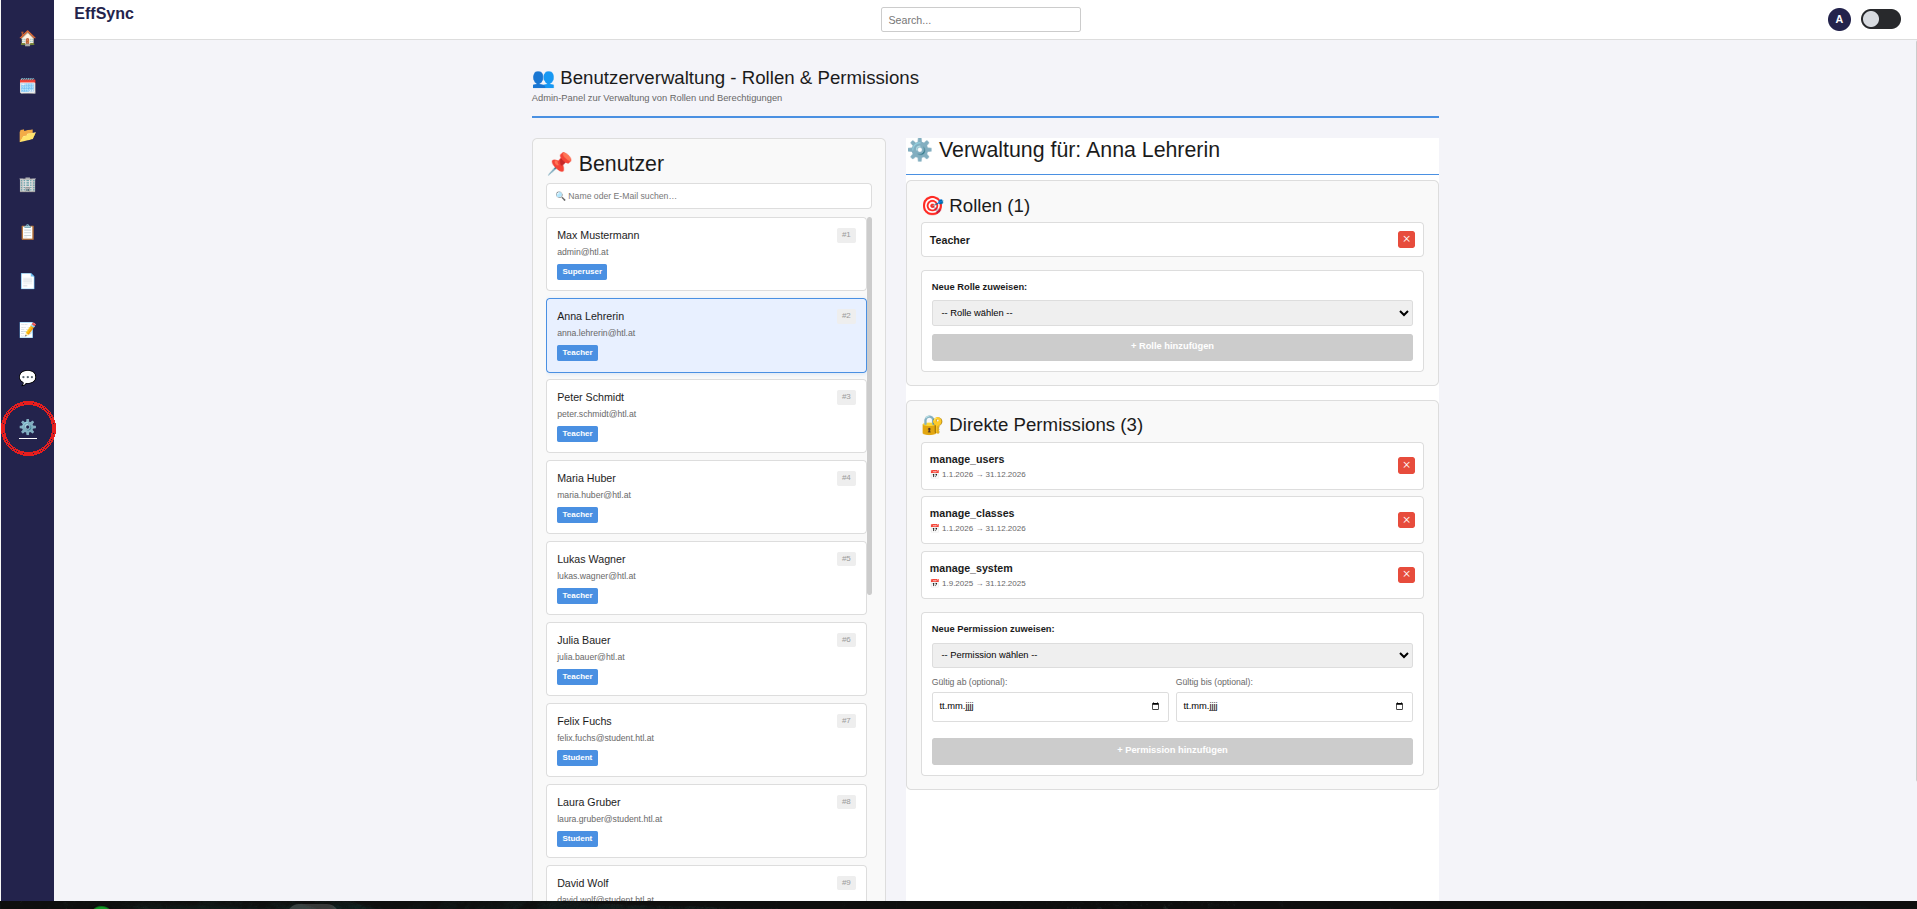
\includegraphics[width=0.95\textwidth]{content/bilder/admin_rollen_permissions.png}
  \caption{Admin-Oberfläche zur Verwaltung von Rollen und Berechtigungen; die rote Markierung zeigt das Zahnrad-Icon in der Seitenleiste, über das der Bereich erreichbar ist}
  \label{fig:admin_rollen_permissions}
\end{figure}

\authorsection{Kommunikation}{Ereny Micail}
\label{sec:kommunikation}
Die Kommunikation wird in \textit{EffSync} als integraler Bestandteil der Projektarbeit umgesetzt. Anstatt auf externe Messenger auszuweichen, erfolgt der Austausch direkt innerhalb der Plattform. Dadurch bleiben Nachrichten im fachlichen Kontext der jeweiligen Aufgaben bzw. Projekträume und sind für alle berechtigten Beteiligten nachvollziehbar.

Für die technische Umsetzung wird auf WebSockets gesetzt, da klassische REST-Schnittstellen keine bidirektionale Echtzeitkommunikation ermöglichen. Das Backend verteilt neue Nachrichten serverseitig per Push-Mechanismus an alle verbundenen Clients eines Raums. Dadurch erscheinen neue Inhalte ohne manuelles Aktualisieren der Benutzeroberfläche.

\authorsection{Benachrichtigungen}{Ereny Micail}
\label{sec:benachrichtigungen}
Benachrichtigungen dienen dazu, relevante Ereignisse unmittelbar sichtbar zu machen, etwa neue Nachrichten, Statusänderungen oder mitgliedschaftsrelevante Aktionen. Die Übertragung erfolgt ereignisgesteuert über die bestehende Echtzeitinfrastruktur. Dadurch reduziert sich die Reaktionszeit der Benutzer deutlich, und kritische Änderungen gehen im Arbeitsfluss nicht verloren.

Aus architektonischer Sicht folgt die Benachrichtigungslogik dem Prinzip, nur fachlich relevante Events zu publizieren. Damit wird unnötige Client-Last vermieden und die Oberfläche bleibt trotz häufiger Ereignisse übersichtlich.

\authorsection{Kalender}{Ereny Micail}
\label{sec:kalender}
Die Kalenderfunktion ergänzt die Aufgabenverwaltung um eine zeitliche Perspektive. Deadlines aus Tasks können in einer kalenderartigen Sicht zusammengeführt werden, wodurch zeitliche Abhängigkeiten und Belastungsspitzen früh erkennbar sind. Dies unterstützt sowohl die individuelle Lernorganisation als auch die Koordination in Teams.

In Verbindung mit Prioritäten und Statusinformationen entsteht eine konsistente Planungsgrundlage: Benutzer sehen nicht nur \textit{was} zu erledigen ist, sondern auch \textit{bis wann} und in welcher Dringlichkeit. Dadurch verbessert die Kalenderintegration die praktische Umsetzbarkeit der zuvor definierten Task-Strukturen.


\authorsection{Taskverwaltung}{Dražen Plavšić}
\label{sec:taskverwaltung}
Da \textit{EffSync} als Task-Management-System konzipiert ist, bildet das Task-Modul das zentrale Element der Anwendung. Die Zielsetzung des Systems ist es, sowohl Schülern als auch Lehrern die Verwaltung von Aufgaben zu erleichtern. Schüler erhalten die Möglichkeit, ihre Aufgaben eigenständig zu organisieren, während Lehrern ein strukturiertes Werkzeug zur Verfügung steht, um Aufgaben gezielt zuzuweisen und deren Bearbeitung zu überwachen.

Das System wurde dabei bewusst über den schulischen Kontext hinaus konzipiert. Durch die Möglichkeit der beliebig tiefen Verschachtelung von Tasks und Subtasks lassen sich nicht nur einfache Aufgaben, sondern auch komplexe Projektstrukturen abbilden. Ein einzelner Task kann dabei ein übergeordnetes Projekt repräsentieren, dessen Teilaufgaben in weitere Unteraufgaben unterteilt werden. Dies macht das Task-Modul von \textit{EffSync} grundsätzlich auch für den unternehmensinternen Einsatz geeignet, da sich ganze Projekte oder Teilprojekte vollständig innerhalb des Systems strukturieren lassen.

\subsection{Datenbankschema und grundlegender Aufbau eines Tasks}{Dražen Plavšić}
Bevor komplexe Mechanismen wie Taskhierarchien und automatische Evaluierungsregeln betrachtet werden, ist es wichtig den grundlegenden strukturellen Aufbau eines \textit{Tasks} zu verstehen. Die Task-Entität bildet das zentrale Kernstück der Applikation und ist in der Datenbank so modelliert, dass sie alle Metadaten für das Projektmanagement effizient speichern kann.

\begin{figure}[H]
  \centering
  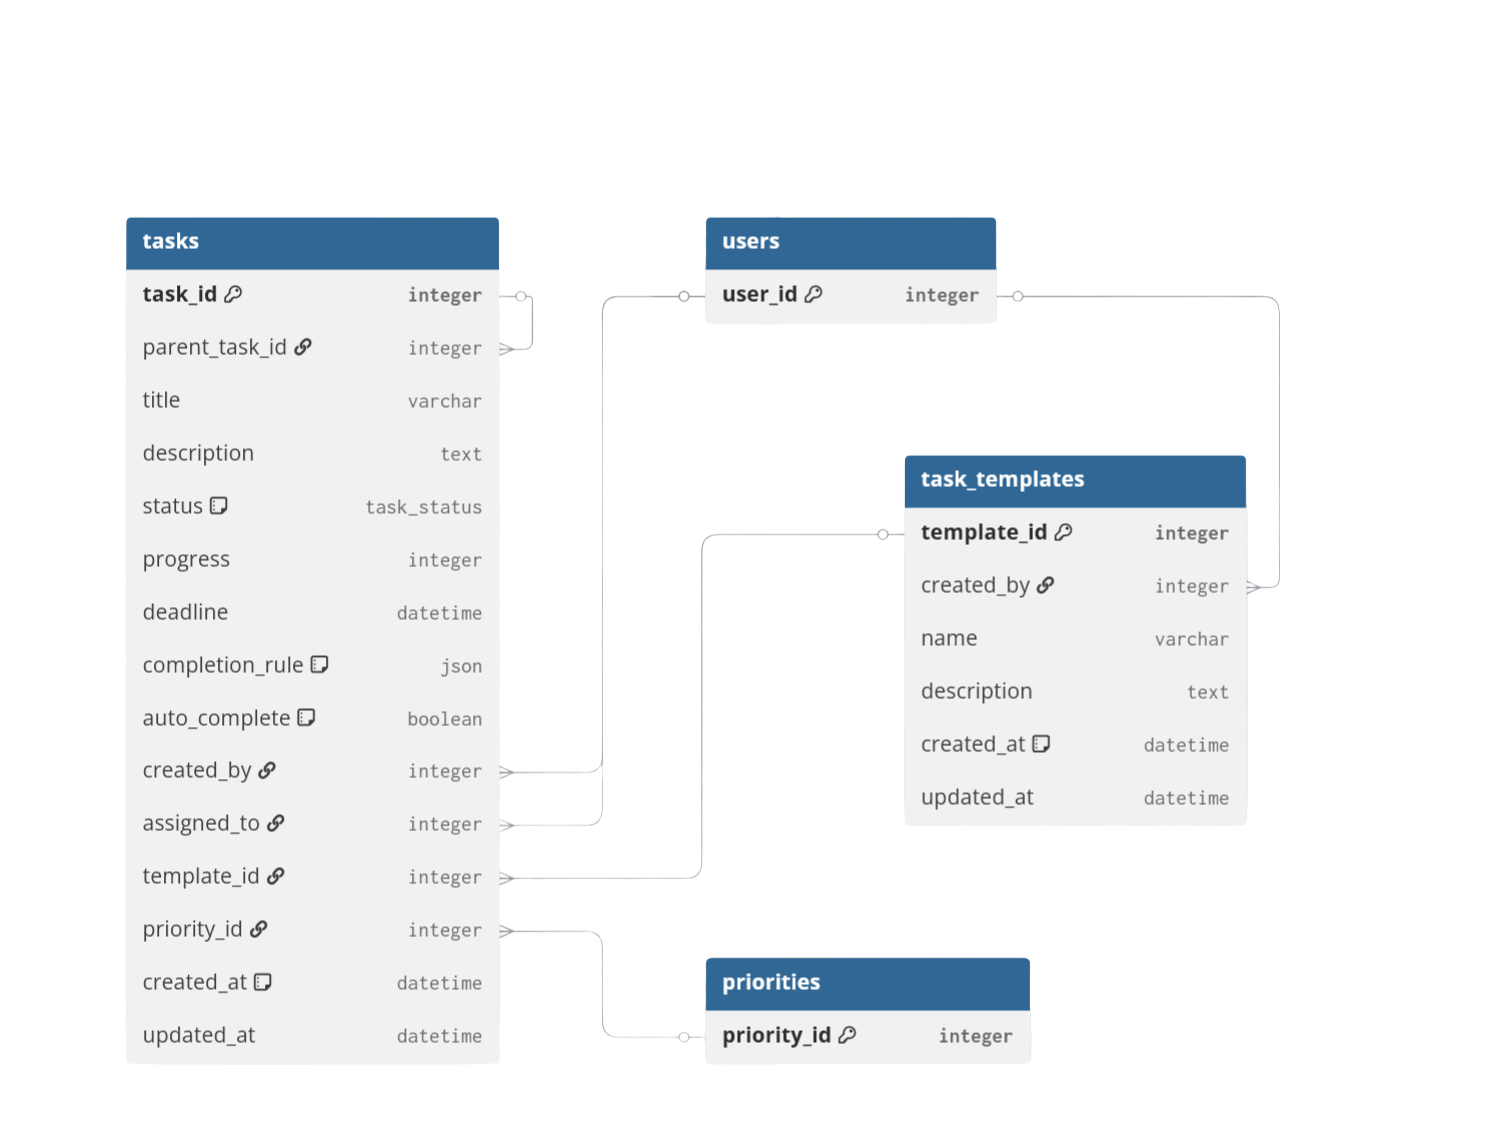
\includegraphics[width=0.8\textwidth]{content/bilder/task_db_schema.png}
  \caption{Auszug des Datenbankschemas zur Verwaltung der Tasks}
  \label{fig:task_schema}
\end{figure}

Die Tasks-Tabelle (siehe Abbildung \ref{fig:task_schema}) lässt sich logisch in drei wesentliche Datenbereiche unterteilen:
\begin{itemize}
    \item \textbf{Basisdaten \& Fortschritt:} Felder wie \texttt{title}, \texttt{description}, \texttt{status} und \texttt{progress} bilden die Kerninformationen für die Benutzeroberfläche. Der Status und der Fortschritt (0 bis 100\,\%) sind logisch aneinander gekoppelt.
    \item \textbf{Verantwortlichkeiten \& Organisation:} Über \texttt{created\_by} und \texttt{assigned\_to} wird auf Datenbankebene sichergestellt, dass jede Aufgabe einem Ersteller und optional einem Bearbeiter zugewiesen ist. Das Feld \texttt{priority\_id} referenziert eine separate Tabelle, um Tasks nach Dringlichkeit (z.\,B. niedrig, hoch) zu kategorisieren, während \texttt{deadline} die zeitliche Frist setzt.
    \item \textbf{Architektonische Steuerungsfelder:} Die Spalte \texttt{parent\_task\_id} dient als Selbstreferenz (\textit{Self-Join}) auf die gleiche Tabelle, um unendlich tiefe Task-Bäume zu ermöglichen. Die Felder \texttt{completion\_rule} (vom Datentyp JSONB) und \texttt{auto\_complete} sind speziell für die eigens entwickelte Rule-Engine reserviert.
\end{itemize}

Dieser Aufbau bildet das Fundament für die gesamte Geschäftslogik der Taskverwaltung, die in den folgenden Abschnitten detailliert erläutert wird.

\subsection{Hierarchie der Tasks}{Dražen Plavšić}
Jeder Task kann über das Feld \texttt{parent\_task\_id} einem übergeordneten Task zugewiesen werden. Dadurch entsteht eine hierarchische Baumstruktur (\textit{Tree Structure})\cite{celko2004trees}, bei der ein Haupt-Task theoretisch unendlich viele Subtasks und deren Nachkommen (\textit{Descendants}) besitzen kann.

Diese strukturelle Flexibilität bringt jedoch eine technische Herausforderung mit sich: die Vermeidung von \textit{Circular References}. Wenn Task A der übergeordnete Task von Task B ist, darf Task B nicht nachträglich als übergeordneter Task von Task A definiert werden. Ebenso darf ein Task nicht sein eigener Parent werden, da dies unweigerlich zu Endlosschleifen beim Auslesen der Daten führen würde.

Um die Datenintegrität aufrechtzuerhalten, implementiert das Backend bei jeder Zuweisung oder Änderung eines Parent-Tasks eine Sicherheitsprüfung. Wie in Listing \ref{lst:circular_reference} dargestellt, traversiert die Methode \texttt{validateNoCircularReference} den Baum iterativ von unten nach oben. Dabei speichert sie alle bereits besuchten Task-IDs in einem \texttt{Set}. Sobald die Methode auf einen Task stößt, dessen ID bereits im Set existiert, greift der Schutzmechanismus und das System bricht den Vorgang mit einer \texttt{BadRequestException} (HTTP Status 400) ab.

\begin{listing}[H]
\begin{minted}{typescript}
// Backend: TasksService
private async validateNoCircularReference(taskId: number, parentTaskId: number): Promise<void> {
  let currentTask = await this.prisma.tasks.findUnique({
    where: { task_id: parentTaskId },
    select: { task_id: true, parent_task_id: true },
  });
  // Set initialisieren, um bereits besuchte Knoten zu speichern
  const visited = new Set<number>([taskId]);
  while (currentTask) {
    if (visited.has(currentTask.task_id)) {
      throw new BadRequestException(
        'Circular reference detected: Task cannot be ancestor of itself'
      );
    }
    visited.add(currentTask.task_id);
    if (!currentTask.parent_task_id) break;
    // Nächsten Knoten in der Hierarchie abfragen
    currentTask = await this.prisma.tasks.findUnique({
      where: { task_id: currentTask.parent_task_id },
      select: { task_id: true, parent_task_id: true },
    });
  }
}
\end{minted}
\caption{Schutz vor Zirkelbezügen durch Traversierung der Baumstruktur}
\label{lst:circular_reference}
\end{listing}

Beim Abrufen der hierarchischen Daten aus der Datenbank nutzt das Backend zwei optimierte Strategien, um verschachtelte Strukturen effizient an das Vue.js-Frontend zu liefern. Für den allgemeinen Listenaufruf sammelt die Hilfsfunktion \texttt{collectDescendants} alle Nachkommen eines Tasks rekursiv über mehrere Datenbankabfragen ein und führt die Ergebnisse im Speicher zusammen. Für die vollständige Baumansicht hingegen werden mit der Methode \texttt{findeOneWithSubtasks} alle relevanten Tasks in \textbf{einer einzigen} Datenbankabfrage geladen und an die \texttt{buildTree} Methode übergeben, welche das Ergebnis serverseitig als tief verschachteltes JSON-Objekt rekonstruiert (siehe Listing \ref{lst:build_tree}).

\begin{listing}[H]
\begin{minted}{typescript}
// Backend: TasksService
async findeOneWithSubtasks(taskId: number, includeRelations = true) {
const rootTask = await this.prisma.tasks.findUnique({
where: { task_id: taskId },
});
// Alle Tasks des Erstellers in einer einzigen Abfrage laden
const allTasks = await this.prisma.tasks.findMany({
where: { created_by: rootTask.created_by },
include: includeRelations ? this.basicInclude() : undefined,
});
// Serverseitige Rekonstruktion als verschachtelter JSON-Baum
return this.buildTree(allTasks, taskId);
}
private buildTree(allTasks: any[], taskId: number) {
const taskMap = new Map();
allTasks.forEach(task =>
taskMap.set(task.task_id, { ...task, subtasks: [] })
);
taskMap.forEach(task => {
const parentTaskId = taskMap.get(task.parent_task_id);
parentTaskId?.subtasks.push(taskMap.get(task.task_id));
});
return taskMap.get(taskId); // Gibt das vollständige JSON-Objekt zurück
}
\end{minted}
\caption{Serverseitige Rekonstruktion des Task-Baums als verschachteltes JSON-Objekt}
\label{lst:build_tree}
\end{listing}

Dieses verschachtelte JSON-Objekt wird anschließend über die \gls{REST-API} direkt an das Vue.js-Frontend übertragen, welches die Struktur ohne weitere Transformationen für die Darstellung der Baumansicht verwenden kann.

\subsection{Rule-Engine und automatische Task-Validierung}{Dražen Plavšić}
\textit{EffSync} besitzt auch die Fähigkeit, übergeordnete Tasks automatisch abzuschließen (\textit{Auto-Completion}), sobald bestimmte vom Nutzer definierte Kriterien der zugehörigen Subtasks erfüllt sind. Um dies zu realisieren, wird eine eigene \textit{Rule-Engine} implementiert, die in einen visuellen Frontend-Builder und einen serverseitigen Evaluator unterteilt ist.

Im Vue.js-Frontend ermöglicht die Komponente \texttt{RuleBuilder} dem Ersteller eines Tasks, logische Bedingungen zu definieren. Dabei können einzelne Subtasks beliebig tief mit logischen Operatoren (\texttt{UND}, \texttt{ODER}, \texttt{XOR}, \texttt{NICHT}) verknüpft werden. Das Frontend übersetzt diese visuelle Darstellung in einen 
\gls{AST} im JSON-Format und übermittelt diesen an das Backend, wo er als \texttt{JSONB}\cite{postgresql_jsonb} abgespeichert wird.

Sobald der Status eines Subtasks geändert wird (beispielsweise auf \texttt{COMPLETED}), löst das Backend einen Event-Trigger aus. Die serverseitige Engine lädt daraufhin den JSONB-Regelbaum des übergeordneten Tasks und wertet diesen aus. Da der Baum beliebig tief verschachtelt sein kann, erfolgt die Auswertung über einen rekursiven Algorithmus.

Wie in Listing~\ref{lst:rule_evaluator} gezeigt, traversiert die Funktion \texttt{evaluateCondition} den JSON-Baum. Handelt es sich bei dem aktuellen Knoten (\textit{Node}) um ein Endblatt (\textit{Leaf}), wird geprüft, ob der referenzierte Task abgeschlossen ist. Handelt es sich hingegen um einen Operator, ruft sich die Funktion für alle angehängten Bedingungen (\textit{Operands}) selbst auf und verknüpft die booleschen Ergebnisse anschließend anhand des jeweiligen logischen Operators.

\begin{listing}[H]
\begin{minted}{typescript}
// Backend: task.evaluator.completion.ts
export function evaluateCondition(
    node: ConditionNode,
    completedTaskIds: Set<string>,
): boolean {
    // Abbruchbedingung der Rekursion: Blattknoten (konkreter Task)
    if (node.type === 'leaf') {
        return completedTaskIds.has(String(node.task_id));
    }
    // Rekursiver Aufruf für alle Kind-Knoten
    const results = node.operands.map(operand =>
        evaluateCondition(operand, completedTaskIds),
    );
    // Auswertung anhand des logischen Operators
    switch (node.operator) {
        case 'AND': return results.every(r => r === true);
        case 'OR':  return results.some(r => r === true);
        case 'XOR': return results.filter(r => r === true).length === 1;
        case 'NOT': return !results[0];
    }
}
\end{minted}
\caption{Rekursive Auswertung des JSONB-Baums zur Task-Validierung}
\label{lst:rule_evaluator}
\end{listing}

Ergibt die Evaluierung des gesamten Baums den Wert \texttt{true}, setzt die Engine den Status des Parent-Tasks automatisch auf \texttt{COMPLETED}. Gleichzeitig wird über das WebSocket-Gateway ein Echtzeit-Event an das Frontend gesendet, um die Benutzeroberfläche aller beteiligten Nutzer ohne Verzögerung zu aktualisieren.

\subsection{Benutzerinteraktion, Usability und Sicherheit}
Neben einer performanten Datenverarbeitung im Hintergrund liegt ein wesentlicher Fokus der Taskverwaltung auf der Benutzerfreundlichkeit (\textit{Usability}) und dem Schutz vor Bedienfehlern im Vue.js-Frontend. 

Um dem Nutzer die Verwaltung einer Vielzahl von Aufgaben zu erleichtern, wird eine dynamische Filter- und Suchfunktion (\texttt{useTaskFilters}) implementiert. Diese ermöglicht es, die Aufgabenliste auf Seiten der Clients, also ohne erneute Datenbankabfrage, in Echtzeit nach Status, Priorität oder Freitext zu filtern und zu sortieren. Die Priorisierung der Aufgaben ist dabei in vier Stufen unterteilt (niedrig, mittel, hoch, dringend), was eine effiziente Arbeitsorganisation unterstützt.

Besonderes Augenmerk wird auf die Datenintegrität und die Vermeidung von ungewolltem Datenverlust gelegt. Das Löschen von Tasks ist daher mit mehrstufigen Sicherheitsmechanismen versehen. Versucht ein Nutzer einen Task zu löschen, der noch aktive Subtasks enthält, lehnt das Backend die Anfrage direkt ab. Dieses Verhalten entspricht dem Prinzip der referentiellen Integrität, bei dem abhängige Kindeinträge das Löschen eines Elterndatensatzes verhindern\cite{postgresql_constraints}. Das System verlangt in diesem Fall zwingend, dass die untergeordneten Aufgaben (\textit{Dependencies}) zuerst gelöscht oder einem anderen Parent-Task zugewiesen werden.

Um zudem versehentliche Löschungen von wichtigen Hauptaufgaben durch simple Fehleingaben (z.\,B.\ durch einen unachtsamen Klick) zu verhindern\cite{uxpsychology_destructive}\cite{nielsen_heuristics}, wurde eine zusätzliche Hürde im Frontend etabliert.

\begin{figure}[H]
  \centering
  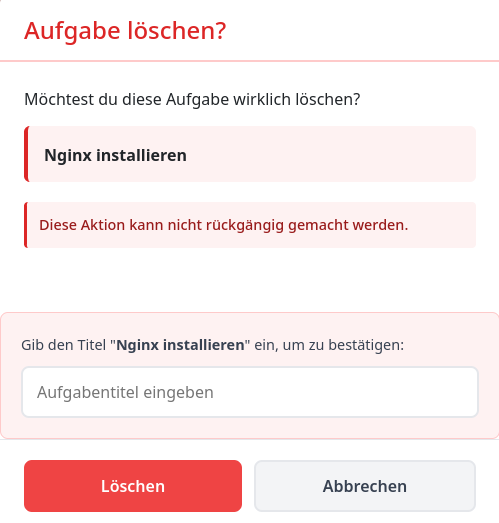
\includegraphics[width=0.4\textwidth]{content/bilder/task_delete_dilog.png}
  \caption{Bestätigungsfenster beim Löschen eines Tasks}
  \label{fig:task_delete}
\end{figure}

Wie Abbildung \ref{fig:task_delete} zeigt, muss der Nutzer bei kritischen Löschvorgängen den exakten Namen des Tasks in ein Dialogfenster abtippen. Erst wenn die Eingabe zeichengenau mit dem Task-Titel übereinstimmt, wird der Lösch-Button freigeschaltet.

Darüber hinaus existieren strikte Prüfungen beim Ändern des Task-Status. Ein Task kann nicht in den Status \texttt{COMPLETED} (Erledigt) übergehen, wenn der verknüpfte Arbeitsfortschritt (\textit{Progress}) noch nicht bei 100\,\% liegt. Auch hier arbeiten Frontend und Backend Hand in Hand: Das UI blockiert die Checkbox visuell, während das Backend bei einem API-Aufruf die Validierung der Werte erzwingt, um inkonsistente Zustände in der Datenbank zu verhindern.

\subsection{Task-Templates zur Effizienzsteigerung}
Da sich viele Arbeitsabläufe, wie beispielsweise Assignments aus Schulfächern (z.\,B.\ POS oder DB), Hausaufgaben für Schüler oder klassische Arbeitspakete in einem Softwareprojekt (z.\,B.\ das Implementieren von Unit-Tests), in ihrer Form und Struktur ähneln und regelmäßig wiederholen, ermöglicht \textit{EffSync} das Abspeichern von Tasks als Vorlage (\textit{Template}). 

Die Verwendung von Vorlagen zur Wiederverwendung wiederkehrender Aufgabenstrukturen ist eine etablierte Praxis in modernen Projektmanagement-Werkzeugen \cite{nielsen_heuristics} und reduziert gemäß dem UX-Prinzip der Effizienz redundante Dateneingaben für erfahrene Nutzer.

Möchte der Nutzer nun einen neuen Arbeitsauftrag erstellen, kann er direkt auf ein gespeichertes Template zurückgreifen. Das Frontend lädt die entsprechenden Parameter aus dem Backend und füllt die Eingabemasken der Benutzeroberfläche automatisch aus. Der Nutzer muss anschließend lediglich aufgabenspezifische, variable Details, wie etwa eine neue Deadline oder eine abweichende Zuweisung (\texttt{assigned\_to}), anpassen, bevor der finale Task generiert wird.

\authorsection{Notizverwaltung}{Ereny Micail}
\label{sec:notizverwaltung}
Die Notizverwaltung erweitert das Task-Modul um eine bewusst einfache Möglichkeit, Informationen schnell und ohne feste Struktur abzulegen. Während Tasks in \textit{EffSync} auf planbare Arbeitseinheiten mit Status, Priorität, Fälligkeit und Zuständigkeiten ausgelegt sind, dienen Notizen als flexibler Zwischenspeicher für Inhalte, die (noch) nicht in ein konkretes Aufgabenmodell passen.

Technisch ist die Notizfunktion als eigenständige Entität umgesetzt, um die strukturierte Aufgabenplanung klar von der freien Textdokumentation zu trennen. Eine Notiz umfasst einen \texttt{title} und eine \texttt{description} und ist eindeutig einem Benutzer zugeordnet. So lassen sich Gedanken, Besprechungsergebnisse, Lehrinhalte oder spontane Ideen ohne zusätzlichen Verwaltungsaufwand erfassen.

Die Geschäftslogik folgt dem bekannten \textit{Create, Read, Update, Delete} (CRUD)-Muster: Nutzer können Notizen anlegen, einsehen, bearbeiten, auflisten und löschen. Anders als bei Tasks wird bewusst auf komplexe Funktionen wie Hierarchien, Fortschrittsmodelle oder automatische Auswertungsregeln verzichtet. Diese Reduktion senkt den Bedienaufwand im Interface und erleichtert die schnelle Erfassung im Arbeitsalltag.

Im Frontend führt dies zu einer schlanken Interaktion: Nach dem Anlegen steht der Notizinhalt sofort bereit und kann bei Bedarf kontinuierlich angepasst werden. Die Notizverwaltung wirkt damit als leichtgewichtiges Pendant zur Taskverwaltung und schließt die Lücke zwischen formaler Aufgabenplanung und informeller Wissenssammlung.

Architektonisch stärkt das Modul die Trennung von Verantwortlichkeiten (\textit{Separation of Concerns}): Tasks bleiben prozessorientiert und auswertbar, Notizen fungieren als freiformorientierter Informationsspeicher. Dadurch steigt die Praxistauglichkeit von \textit{EffSync}, weil Informationen nicht zwanghaft in die starre Struktur eines Tasks gepresst werden müssen.

\authorsection{Live-Chat}{Dražen Plavšić}
\label{sec:live_chat}

Im akademischen Umfeld der HTL, aber auch in der modernen Softwareindustrie zeigt sich bei der Projektarbeit häufig ein wiederkehrendes Problem: Etablierte Task-Management-Lösungen bieten meist keine native, integrierte Echtzeitkommunikation\cite{trello_powerup_boardchat}\cite{atlassian_jira_11_3_documentation}\cite{atlassian_trello_guide}\cite{atlassian_trello_tour}. Dies zwingt Arbeitsgruppen dazu für Absprachen auf externe Kommunikationsplattformen wie Discord, Slack, WhatsApp oder Microsoft Teams auszuweichen. Dieser ständige Plattformwechsel (\textit{Context Switching}) führt zu einem fragmentierten Informationsfluss, bei dem Projektkontext und Aufgabenbezug schnell verloren gehen. 

Um dieses Problem zu lösen, wird in \textit{EffSync} ein nativer Live-Chat implementiert. Diese nahtlose Verschmelzung von Aufgabenverwaltung und Echtzeitkommunikation stellt die \textit{Unique Selling Proposition} (USP) der Applikation dar. 

\subsection{Technologische Umsetzung mittels WebSockets}
Da klassische REST-Schnittstellen auf dem Request-Response-Prinzip basieren, eignen sie sich nicht für Echtzeitanwendungen, da sie keine serverseitige Push-Kommunikation unterstützen~\cite{websocket_restapi_hybrid}. Ein ständiges Abfragen des Servers (\textit{HTTP-Polling}) nach neuen Nachrichten würde zudem unnötige Netzwerklast erzeugen, da jede HTTP-Anfrage einen erheblichen Protokoll-Overhead mit sich bringt~\cite{diva_polling_ws_2017}. Daher wird die Chat-Funktion vollständig über \textit{WebSockets} realisiert. Im Backend kommen hierbei NestJS-Gateways zum Einsatz, welche eine dauerhafte, bidirektionale Verbindung zum Vue-Frontend aufrechterhalten. Sendet ein Nutzer eine Nachricht, wird diese vom Server validiert und in Echtzeit per Push-Verfahren an alle relevanten Clients im jeweiligen Chatraum (\textit{Room}) verteilt (siehe Abbildung \ref{fig:datenfluss_websocket}).
\begin{figure}[H]
  \centering
  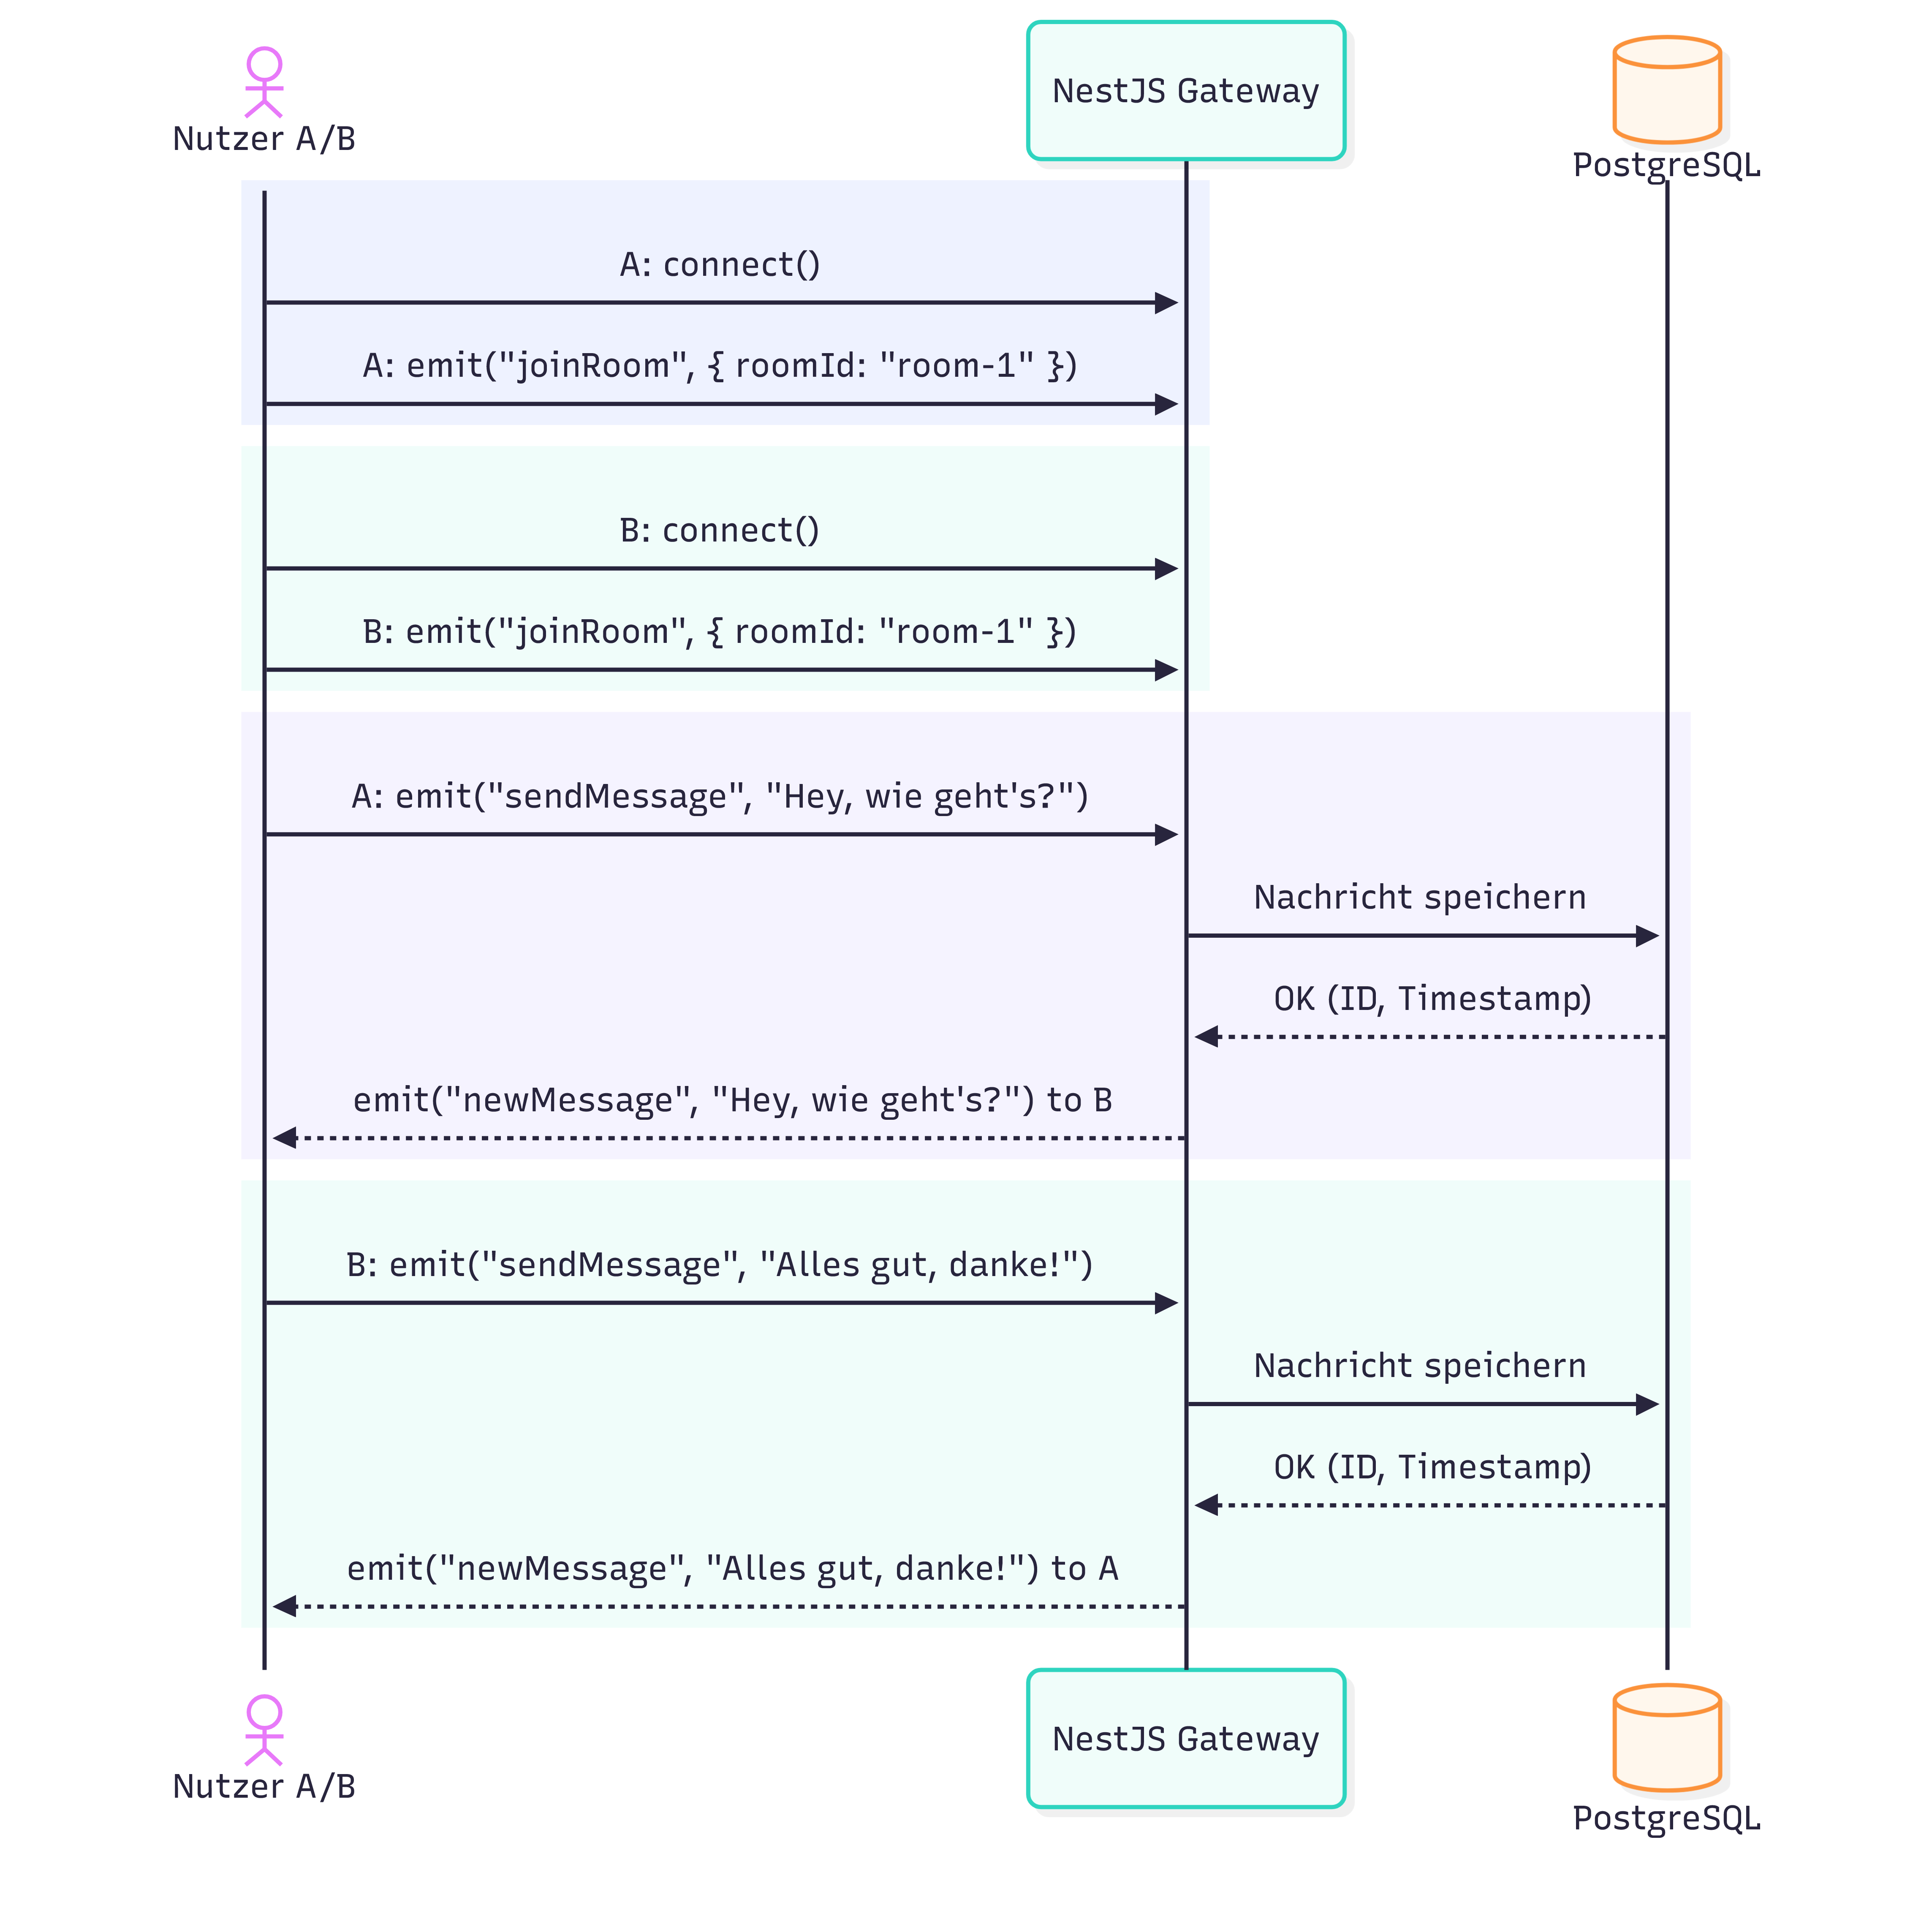
\includegraphics[width=0.6\textwidth]{content/bilder/realtime_chat_simpler_no_notes.png}
  \caption{Echtzeit-Datenfluss via WebSockets}
  \label{fig:datenfluss_websocket}
\end{figure}

\subsection{Unterscheidung der Chat-Typen und Vermeidung von Duplikaten}
In \textit{EffSync} wird das Chat-System prinzipiell in zwei Raumtypen (\textit{Rooms}) unterteilt: private 1-zu-1-Chats und projektbezogene Gruppenchats. Diese Unterscheidung ist nicht nur für die Darstellung in der Benutzeroberfläche relevant, sondern vor allem für die Datenmodellierung und die Berechtigungslogik wichtig. 

Wie im Datenbankschema (siehe Abbildung \ref{fig:chat_schema}) zu erkennen ist, wird der Raumtyp über das Flag \texttt{is\_private} in der Tabelle \texttt{chat\_rooms} gesteuert. Bei Gruppenchats kann zudem optional eine direkte Verknüpfung zur entsprechenden Aufgabe (\texttt{task\_id}) hergestellt werden.

\begin{figure}[H]
    \centering
    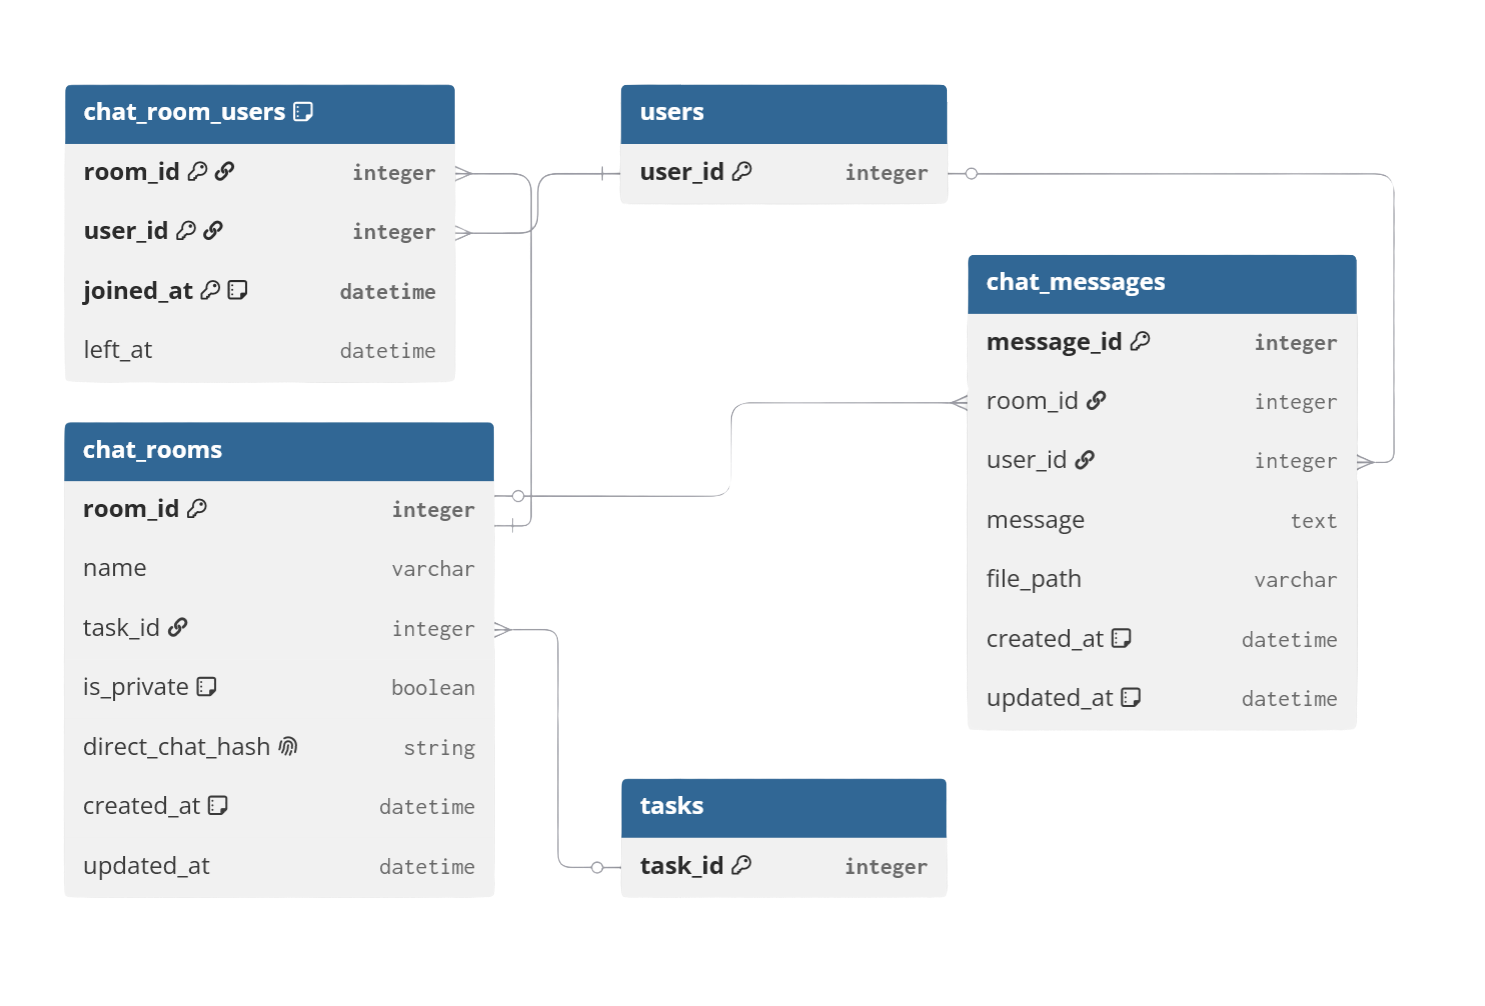
\includegraphics[width=0.8\textwidth]{content/bilder/chat_db_schema.png}
    \caption{Auszug des Datenbankschemas zur Verwaltung der Chaträume}
    \label{fig:chat_schema}
\end{figure}

Bei der Initialisierung von privaten Chats greift serverseitig eine spezielle Validierungslogik, um die Erstellung redundanter Chaträume zu verhindern. Möchte Nutzer A einen Chat mit Nutzer B starten, muss sichergestellt werden, dass für diese Konstellation nicht bereits ein Raum existiert. Anstatt hierfür eine rechenintensive Datenbankabfrage über die Mitgliedertabelle durchzuführen, wird dies über das Feld \texttt{direct\_chat\_hash} in der Tabelle \texttt{chat\_rooms} (siehe Abbildung \ref{fig:chat_schema}) gelöst. 

Aus den Identifikationsnummern der beiden Teilnehmer wird ein deterministischer String generiert (beispielsweise \texttt{user1\_user2}). Da dieses Feld in der Datenbank mit einem \texttt{UNIQUE}-Constraint versehen ist, wird die Erstellung eines Duplikats bereits auf Datenbankebene strikt abgelehnt. Schlägt der Erstellungsversuch aufgrund des Constraints fehl, wird die Erstellung blockiert und dem Client stattdessen die ID des bestehenden Raums zurückgegeben. Dies garantiert, dass die Konversation zwischen zwei Personen nicht fragmentiert wird, sondern die gesamte Historie stets in einem einzigen, fortlaufenden Chatverlauf bleibt.

\subsection{Raumverwaltung und Berechtigungslogik}
Während in einem privaten Chat beide Teilnehmer gleichgestellte Rechte besitzen, erfordern Gruppenchats eine hierarchische Rollenverteilung, um administrative Aufgaben abzubilden. Die Komplexität liegt hierbei in der sicheren Verwaltung der Zugriffsrechte (\textit{Authorization}). Ein exemplarisches Sicherheitsszenario ist das Entfernen von Mitgliedern aus einem Gruppenchat. 

Wie in Listing~\ref{lst:chat_permissions} dargestellt, wurde im Backend eine strikte Berechtigungslogik implementiert, die bei Modifikationen der Raummitglieder zwischen zwei Szenarien unterscheidet: Möchte ein Nutzer den Chatraum freiwillig verlassen (\texttt{requesterId === targetUserId}), wird die Aktion ohne weitere Prüfung gestattet. Versucht jedoch ein Nutzer eine andere Person aus dem Gruppenraum zu entfernen, greift eine Sicherheitsprüfung (\texttt{assertIsCreator}). Diese stellt sicher, dass ausschließlich der ursprüngliche Ersteller des Chatraums das Recht besitzt, andere Mitglieder auszuschließen. Andernfalls meldet das System aus Sicherheitsgründen sofort eine \texttt{ForbiddenException} (HTTP Status 403).

\begin{listing}[H]
\begin{minted}{typescript}
// Backend: ChatRoomsService
async removeMember(roomId: number, requesterId: number, targetUserId: number) {
    // Szenario B: User versucht jemand anderen zu entfernen
    if (requesterId !== targetUserId) {
        // Prüft, ob der Requester der Creator des Gruppenraums ist. 
        // Wirft intern eine ForbiddenException, falls nicht.
        await this.chatRoomsService.assertIsCreator(roomId, requesterId);
    }
    // Szenario A (User entfernt sich selbst) oder
    // Szenario B (Creator entfernt User) war erfolgreich:
    return this.chatRoomMembersRepository.delete({ roomId, userId: targetUserId });
}
async assertIsCreator(roomId: number, userId: number) {
    // Raum anhand der roomId aus der Datenbank laden,
    // nur das Feld created_by wird benötigt.
    const room = await this.prisma.chat_rooms.findUnique({
        where: { room_id: roomId },
        select: { created_by: true },
    });
    // Raum existiert nicht → 404
    if (!room) throw new NotFoundException('Room not found!');
    // Prüft, ob der anfragende User der Ersteller des Raums ist.
    // Falls nicht → 403 ForbiddenException
    if (room.created_by !== userId)
        throw new ForbiddenException('Only the room creator can do this!');
}
\end{minted}
\caption{Berechtigungsprüfung beim Entfernen von Mitgliedern aus einem Gruppenchat}
\label{lst:chat_permissions}
\end{listing}